% Created by tikzDevice version 0.12.6 on 2026-07-04 06:01:32
% !TEX encoding = UTF-8 Unicode
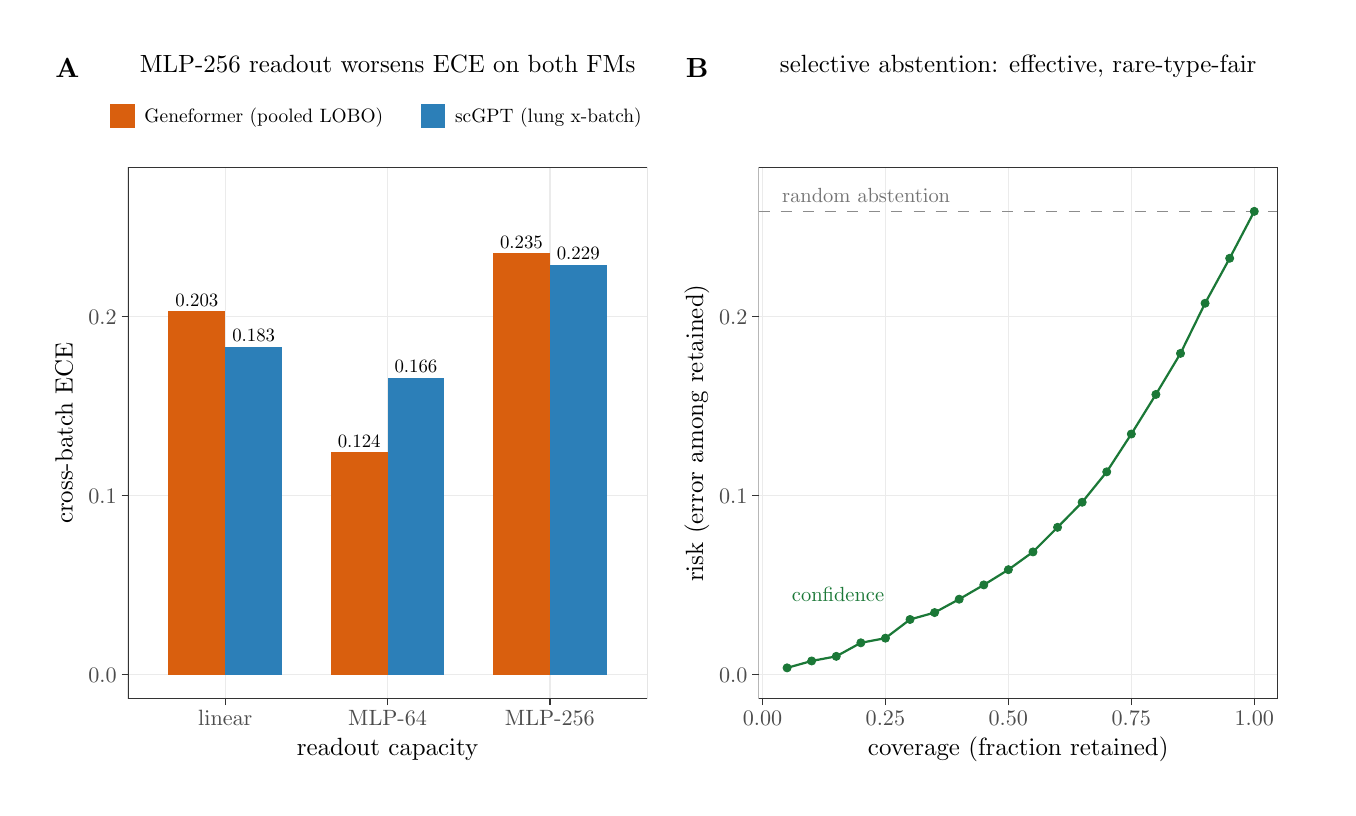
\begin{tikzpicture}[x=1pt,y=1pt]
\definecolor{fillColor}{RGB}{255,255,255}
\path[use as bounding box,fill=fillColor,fill opacity=0.00] (0,0) rectangle (469.75,274.63);
\begin{scope}
\path[clip] (  0.00,  0.00) rectangle (469.75,274.63);
\definecolor{drawColor}{RGB}{255,255,255}
\definecolor{fillColor}{RGB}{255,255,255}

\path[draw=drawColor,line width= 0.5pt,line join=round,line cap=round,fill=fillColor] (  0.00,  0.00) rectangle (469.75,274.63);
\end{scope}
\begin{scope}
\path[clip] (  5.00,  5.00) rectangle (232.88,269.63);
\definecolor{drawColor}{RGB}{255,255,255}
\definecolor{fillColor}{RGB}{255,255,255}

\path[draw=drawColor,line width= 0.5pt,line join=round,line cap=round,fill=fillColor] (  5.00,  5.00) rectangle (232.88,269.63);
\end{scope}
\begin{scope}
\path[clip] (232.88,  5.00) rectangle (460.75,269.63);
\definecolor{drawColor}{RGB}{255,255,255}
\definecolor{fillColor}{RGB}{255,255,255}

\path[draw=drawColor,line width= 0.5pt,line join=round,line cap=round,fill=fillColor] (232.88,  5.00) rectangle (460.76,269.63);
\end{scope}
\begin{scope}
\path[clip] ( 36.22, 32.07) rectangle (223.88,224.18);
\definecolor{fillColor}{RGB}{255,255,255}

\path[fill=fillColor] ( 36.22, 32.07) rectangle (223.88,224.18);
\definecolor{drawColor}{gray}{0.92}

\path[draw=drawColor,line width= 0.5pt,line join=round] ( 36.22, 40.80) --
	(223.88, 40.80);

\path[draw=drawColor,line width= 0.5pt,line join=round] ( 36.22,105.48) --
	(223.88,105.48);

\path[draw=drawColor,line width= 0.5pt,line join=round] ( 36.22,170.17) --
	(223.88,170.17);

\path[draw=drawColor,line width= 0.5pt,line join=round] ( 71.41, 32.07) --
	( 71.41,224.18);

\path[draw=drawColor,line width= 0.5pt,line join=round] (130.05, 32.07) --
	(130.05,224.18);

\path[draw=drawColor,line width= 0.5pt,line join=round] (188.69, 32.07) --
	(188.69,224.18);
\definecolor{fillColor}{RGB}{44,127,184}

\path[fill=fillColor] ( 71.41, 40.80) rectangle ( 91.93,159.17);

\path[fill=fillColor] (130.05, 40.80) rectangle (150.57,148.17);

\path[fill=fillColor] (188.69, 40.80) rectangle (209.22,188.92);
\definecolor{fillColor}{RGB}{217,95,14}

\path[fill=fillColor] ( 50.88, 40.80) rectangle ( 71.41,172.17);

\path[fill=fillColor] (109.52, 40.80) rectangle (130.05,121.14);

\path[fill=fillColor] (168.17, 40.80) rectangle (188.69,193.13);
\definecolor{drawColor}{RGB}{0,0,0}

\node[text=drawColor,anchor=base,inner sep=0pt, outer sep=0pt, scale=  0.68] at ( 81.67,161.05) {0.183};

\node[text=drawColor,anchor=base,inner sep=0pt, outer sep=0pt, scale=  0.68] at (140.31,150.05) {0.166};

\node[text=drawColor,anchor=base,inner sep=0pt, outer sep=0pt, scale=  0.68] at (198.95,190.81) {0.229};

\node[text=drawColor,anchor=base,inner sep=0pt, outer sep=0pt, scale=  0.68] at ( 61.15,174.05) {0.203};

\node[text=drawColor,anchor=base,inner sep=0pt, outer sep=0pt, scale=  0.68] at (119.79,123.02) {0.124};

\node[text=drawColor,anchor=base,inner sep=0pt, outer sep=0pt, scale=  0.68] at (178.43,195.01) {0.235};
\definecolor{drawColor}{gray}{0.20}

\path[draw=drawColor,line width= 0.5pt,line join=round,line cap=round] ( 36.22, 32.07) rectangle (223.88,224.18);
\end{scope}
\begin{scope}
\path[clip] (  0.00,  0.00) rectangle (469.75,274.63);
\definecolor{drawColor}{gray}{0.30}

\node[text=drawColor,anchor=base east,inner sep=0pt, outer sep=0pt, scale=  0.80] at ( 32.17, 38.04) {0.0};

\node[text=drawColor,anchor=base east,inner sep=0pt, outer sep=0pt, scale=  0.80] at ( 32.17,102.73) {0.1};

\node[text=drawColor,anchor=base east,inner sep=0pt, outer sep=0pt, scale=  0.80] at ( 32.17,167.41) {0.2};
\end{scope}
\begin{scope}
\path[clip] (  0.00,  0.00) rectangle (469.75,274.63);
\definecolor{drawColor}{gray}{0.20}

\path[draw=drawColor,line width= 0.5pt,line join=round] ( 33.97, 40.80) --
	( 36.22, 40.80);

\path[draw=drawColor,line width= 0.5pt,line join=round] ( 33.97,105.48) --
	( 36.22,105.48);

\path[draw=drawColor,line width= 0.5pt,line join=round] ( 33.97,170.17) --
	( 36.22,170.17);
\end{scope}
\begin{scope}
\path[clip] (  0.00,  0.00) rectangle (469.75,274.63);
\definecolor{drawColor}{gray}{0.20}

\path[draw=drawColor,line width= 0.5pt,line join=round] ( 71.41, 29.82) --
	( 71.41, 32.07);

\path[draw=drawColor,line width= 0.5pt,line join=round] (130.05, 29.82) --
	(130.05, 32.07);

\path[draw=drawColor,line width= 0.5pt,line join=round] (188.69, 29.82) --
	(188.69, 32.07);
\end{scope}
\begin{scope}
\path[clip] (  0.00,  0.00) rectangle (469.75,274.63);
\definecolor{drawColor}{gray}{0.30}

\node[text=drawColor,anchor=base,inner sep=0pt, outer sep=0pt, scale=  0.80] at ( 71.41, 22.51) {linear};

\node[text=drawColor,anchor=base,inner sep=0pt, outer sep=0pt, scale=  0.80] at (130.05, 22.51) {MLP-64};

\node[text=drawColor,anchor=base,inner sep=0pt, outer sep=0pt, scale=  0.80] at (188.69, 22.51) {MLP-256};
\end{scope}
\begin{scope}
\path[clip] (  0.00,  0.00) rectangle (469.75,274.63);
\definecolor{drawColor}{RGB}{0,0,0}

\node[text=drawColor,anchor=base,inner sep=0pt, outer sep=0pt, scale=  0.90] at (130.05, 11.75) {readout capacity};
\end{scope}
\begin{scope}
\path[clip] (  0.00,  0.00) rectangle (469.75,274.63);
\definecolor{drawColor}{RGB}{0,0,0}

\node[text=drawColor,rotate= 90.00,anchor=base,inner sep=0pt, outer sep=0pt, scale=  0.90] at ( 16.20,128.12) {cross-batch ECE};
\end{scope}
\begin{scope}
\path[clip] (  0.00,  0.00) rectangle (469.75,274.63);
\definecolor{fillColor}{RGB}{255,255,255}

\path[fill=fillColor] ( 24.71,233.18) rectangle (235.39,252.18);
\end{scope}
\begin{scope}
\path[clip] (  0.00,  0.00) rectangle (469.75,274.63);
\definecolor{fillColor}{RGB}{255,255,255}

\path[fill=fillColor] ( 29.21,237.68) rectangle ( 39.21,247.68);
\definecolor{fillColor}{RGB}{217,95,14}

\path[fill=fillColor] ( 29.79,238.26) rectangle ( 38.62,247.09);
\end{scope}
\begin{scope}
\path[clip] (  0.00,  0.00) rectangle (469.75,274.63);
\definecolor{fillColor}{RGB}{255,255,255}

\path[fill=fillColor] (141.43,237.68) rectangle (151.43,247.68);
\definecolor{fillColor}{RGB}{44,127,184}

\path[fill=fillColor] (142.01,238.26) rectangle (150.85,247.09);
\end{scope}
\begin{scope}
\path[clip] (  0.00,  0.00) rectangle (469.75,274.63);
\definecolor{drawColor}{RGB}{0,0,0}

\node[text=drawColor,anchor=base west,inner sep=0pt, outer sep=0pt, scale=  0.70] at ( 42.21,240.27) {Geneformer (pooled LOBO)};
\end{scope}
\begin{scope}
\path[clip] (  0.00,  0.00) rectangle (469.75,274.63);
\definecolor{drawColor}{RGB}{0,0,0}

\node[text=drawColor,anchor=base west,inner sep=0pt, outer sep=0pt, scale=  0.70] at (154.43,240.27) {scGPT (lung x-batch)};
\end{scope}
\begin{scope}
\path[clip] (  0.00,  0.00) rectangle (469.75,274.63);
\definecolor{drawColor}{RGB}{0,0,0}

\node[text=drawColor,anchor=base,inner sep=0pt, outer sep=0pt, scale=  0.90] at (130.05,258.43) {MLP-256 readout worsens ECE on both FMs};
\end{scope}
\begin{scope}
\path[clip] (  0.00,  0.00) rectangle (469.75,274.63);
\definecolor{drawColor}{RGB}{0,0,0}

\node[text=drawColor,anchor=base,inner sep=0pt, outer sep=0pt, scale=  1.00] at ( 14.35,256.66) {\bfseries A};
\end{scope}
\begin{scope}
\path[clip] (264.10, 32.07) rectangle (451.75,224.18);
\definecolor{fillColor}{RGB}{255,255,255}

\path[fill=fillColor] (264.10, 32.07) rectangle (451.75,224.18);
\definecolor{drawColor}{gray}{0.92}

\path[draw=drawColor,line width= 0.5pt,line join=round] (264.10, 40.80) --
	(451.75, 40.80);

\path[draw=drawColor,line width= 0.5pt,line join=round] (264.10,105.48) --
	(451.75,105.48);

\path[draw=drawColor,line width= 0.5pt,line join=round] (264.10,170.17) --
	(451.75,170.17);

\path[draw=drawColor,line width= 0.5pt,line join=round] (265.52, 32.07) --
	(265.52,224.18);

\path[draw=drawColor,line width= 0.5pt,line join=round] (309.95, 32.07) --
	(309.95,224.18);

\path[draw=drawColor,line width= 0.5pt,line join=round] (354.37, 32.07) --
	(354.37,224.18);

\path[draw=drawColor,line width= 0.5pt,line join=round] (398.80, 32.07) --
	(398.80,224.18);

\path[draw=drawColor,line width= 0.5pt,line join=round] (443.23, 32.07) --
	(443.23,224.18);
\definecolor{drawColor}{gray}{0.55}

\path[draw=drawColor,line width= 0.5pt,dash pattern=on 4pt off 4pt ,line join=round] (264.10,208.26) -- (451.75,208.26);
\definecolor{drawColor}{gray}{0.45}

\node[text=drawColor,anchor=base west,inner sep=0pt, outer sep=0pt, scale=  0.74] at (272.63,211.54) {random abstention};
\definecolor{drawColor}{RGB}{27,120,55}

\path[draw=drawColor,line width= 0.8pt,line join=round] (274.41, 43.30) --
	(283.29, 45.79) --
	(292.18, 47.46) --
	(301.06, 52.35) --
	(309.95, 54.03) --
	(318.83, 60.78) --
	(327.72, 63.28) --
	(336.60, 68.11) --
	(345.49, 73.27) --
	(354.37, 78.77) --
	(363.26, 85.19) --
	(372.14, 94.08) --
	(381.03,103.14) --
	(389.91,114.13) --
	(398.80,127.79) --
	(407.68,142.10) --
	(416.57,156.93) --
	(425.45,175.04) --
	(434.34,191.30) --
	(443.23,208.25);
\definecolor{fillColor}{RGB}{27,120,55}

\path[draw=drawColor,line width= 0.3pt,line join=round,line cap=round,fill=fillColor] (274.41, 43.30) circle (  1.47);

\path[draw=drawColor,line width= 0.3pt,line join=round,line cap=round,fill=fillColor] (283.29, 45.79) circle (  1.47);

\path[draw=drawColor,line width= 0.3pt,line join=round,line cap=round,fill=fillColor] (292.18, 47.46) circle (  1.47);

\path[draw=drawColor,line width= 0.3pt,line join=round,line cap=round,fill=fillColor] (301.06, 52.35) circle (  1.47);

\path[draw=drawColor,line width= 0.3pt,line join=round,line cap=round,fill=fillColor] (309.95, 54.03) circle (  1.47);

\path[draw=drawColor,line width= 0.3pt,line join=round,line cap=round,fill=fillColor] (318.83, 60.78) circle (  1.47);

\path[draw=drawColor,line width= 0.3pt,line join=round,line cap=round,fill=fillColor] (327.72, 63.28) circle (  1.47);

\path[draw=drawColor,line width= 0.3pt,line join=round,line cap=round,fill=fillColor] (336.60, 68.11) circle (  1.47);

\path[draw=drawColor,line width= 0.3pt,line join=round,line cap=round,fill=fillColor] (345.49, 73.27) circle (  1.47);

\path[draw=drawColor,line width= 0.3pt,line join=round,line cap=round,fill=fillColor] (354.37, 78.77) circle (  1.47);

\path[draw=drawColor,line width= 0.3pt,line join=round,line cap=round,fill=fillColor] (363.26, 85.19) circle (  1.47);

\path[draw=drawColor,line width= 0.3pt,line join=round,line cap=round,fill=fillColor] (372.14, 94.08) circle (  1.47);

\path[draw=drawColor,line width= 0.3pt,line join=round,line cap=round,fill=fillColor] (381.03,103.14) circle (  1.47);

\path[draw=drawColor,line width= 0.3pt,line join=round,line cap=round,fill=fillColor] (389.91,114.13) circle (  1.47);

\path[draw=drawColor,line width= 0.3pt,line join=round,line cap=round,fill=fillColor] (398.80,127.79) circle (  1.47);

\path[draw=drawColor,line width= 0.3pt,line join=round,line cap=round,fill=fillColor] (407.68,142.10) circle (  1.47);

\path[draw=drawColor,line width= 0.3pt,line join=round,line cap=round,fill=fillColor] (416.57,156.93) circle (  1.47);

\path[draw=drawColor,line width= 0.3pt,line join=round,line cap=round,fill=fillColor] (425.45,175.04) circle (  1.47);

\path[draw=drawColor,line width= 0.3pt,line join=round,line cap=round,fill=fillColor] (434.34,191.30) circle (  1.47);

\path[draw=drawColor,line width= 0.3pt,line join=round,line cap=round,fill=fillColor] (443.23,208.25) circle (  1.47);

\node[text=drawColor,anchor=base west,inner sep=0pt, outer sep=0pt, scale=  0.74] at (276.18, 67.36) {confidence};
\definecolor{drawColor}{gray}{0.20}

\path[draw=drawColor,line width= 0.5pt,line join=round,line cap=round] (264.10, 32.07) rectangle (451.75,224.18);
\end{scope}
\begin{scope}
\path[clip] (  0.00,  0.00) rectangle (469.75,274.63);
\definecolor{drawColor}{gray}{0.30}

\node[text=drawColor,anchor=base east,inner sep=0pt, outer sep=0pt, scale=  0.80] at (260.05, 38.04) {0.0};

\node[text=drawColor,anchor=base east,inner sep=0pt, outer sep=0pt, scale=  0.80] at (260.05,102.73) {0.1};

\node[text=drawColor,anchor=base east,inner sep=0pt, outer sep=0pt, scale=  0.80] at (260.05,167.41) {0.2};
\end{scope}
\begin{scope}
\path[clip] (  0.00,  0.00) rectangle (469.75,274.63);
\definecolor{drawColor}{gray}{0.20}

\path[draw=drawColor,line width= 0.5pt,line join=round] (261.85, 40.80) --
	(264.10, 40.80);

\path[draw=drawColor,line width= 0.5pt,line join=round] (261.85,105.48) --
	(264.10,105.48);

\path[draw=drawColor,line width= 0.5pt,line join=round] (261.85,170.17) --
	(264.10,170.17);
\end{scope}
\begin{scope}
\path[clip] (  0.00,  0.00) rectangle (469.75,274.63);
\definecolor{drawColor}{gray}{0.20}

\path[draw=drawColor,line width= 0.5pt,line join=round] (265.52, 29.82) --
	(265.52, 32.07);

\path[draw=drawColor,line width= 0.5pt,line join=round] (309.95, 29.82) --
	(309.95, 32.07);

\path[draw=drawColor,line width= 0.5pt,line join=round] (354.37, 29.82) --
	(354.37, 32.07);

\path[draw=drawColor,line width= 0.5pt,line join=round] (398.80, 29.82) --
	(398.80, 32.07);

\path[draw=drawColor,line width= 0.5pt,line join=round] (443.23, 29.82) --
	(443.23, 32.07);
\end{scope}
\begin{scope}
\path[clip] (  0.00,  0.00) rectangle (469.75,274.63);
\definecolor{drawColor}{gray}{0.30}

\node[text=drawColor,anchor=base,inner sep=0pt, outer sep=0pt, scale=  0.80] at (265.52, 22.51) {0.00};

\node[text=drawColor,anchor=base,inner sep=0pt, outer sep=0pt, scale=  0.80] at (309.95, 22.51) {0.25};

\node[text=drawColor,anchor=base,inner sep=0pt, outer sep=0pt, scale=  0.80] at (354.37, 22.51) {0.50};

\node[text=drawColor,anchor=base,inner sep=0pt, outer sep=0pt, scale=  0.80] at (398.80, 22.51) {0.75};

\node[text=drawColor,anchor=base,inner sep=0pt, outer sep=0pt, scale=  0.80] at (443.23, 22.51) {1.00};
\end{scope}
\begin{scope}
\path[clip] (  0.00,  0.00) rectangle (469.75,274.63);
\definecolor{drawColor}{RGB}{0,0,0}

\node[text=drawColor,anchor=base,inner sep=0pt, outer sep=0pt, scale=  0.90] at (357.93, 11.75) {coverage (fraction retained)};
\end{scope}
\begin{scope}
\path[clip] (  0.00,  0.00) rectangle (469.75,274.63);
\definecolor{drawColor}{RGB}{0,0,0}

\node[text=drawColor,rotate= 90.00,anchor=base,inner sep=0pt, outer sep=0pt, scale=  0.90] at (244.08,128.12) {risk (error among retained)};
\end{scope}
\begin{scope}
\path[clip] (  0.00,  0.00) rectangle (469.75,274.63);
\definecolor{drawColor}{RGB}{0,0,0}

\node[text=drawColor,anchor=base,inner sep=0pt, outer sep=0pt, scale=  0.90] at (357.93,258.43) {selective abstention: effective, rare-type-fair};
\end{scope}
\begin{scope}
\path[clip] (  0.00,  0.00) rectangle (469.75,274.63);
\definecolor{drawColor}{RGB}{0,0,0}

\node[text=drawColor,anchor=base,inner sep=0pt, outer sep=0pt, scale=  1.00] at (241.97,256.66) {\bfseries B};
\end{scope}
\end{tikzpicture}
